% !TeX root = ../main.tex
% Add the above to each chapter to make compiling the PDF easier in some editors.

\chapter{Probability}

\section{Random Walks}

In this section, we study random walks on undirected weighted graphs $G = (\sV, \sE, \vw)$ with self-loops. A \emph{random walk}\index{random walk} visits a random sequence of vertices $X_1, X_2, \dots$, where \begin{align}
    \Pr{X_{t+1} = v \mid X_t = u} = \frac{\vw(\{v, u\})}{\vd(u)}
\end{align} and $\vd(u)$ is the weighted degree of vertex $u$, as we have defined previously.

\begin{rmk}
The random walks considered here satisfy the \emph{Markov property}\index{Markov property}, that is, \begin{align}
    X_{t+1} \perp X_1, \dots, X_{t-1} \mid X_t.\safefootnote{So you can think of these random walks as Markov chains.}
\end{align} Moreover, we restrict our attention to time-homogeneous random walks, that is, the transition probabilities remain constant over time.
\end{rmk}

We can therefore model the update of a single round using the linear map $\mW \in \R^{|\sV|\times|\sV|}$ (called \emph{transition matrix}\index{transition matrix}), \begin{align}
    \mW \defeq \begin{bmatrix}
    \frac{\vw(\{1,1\})}{\vd(1)} & \cdots & \frac{\vw(\{n, 1\})}{\vd(n)} \\
    \vdots & \ddots & \vdots \\
    \frac{\vw(\{1,n\})}{\vd(1)} & \cdots & \frac{\vw(\{n, n\})}{\vd(n)} \\
    \end{bmatrix} = \mA\inv{\mD}.
\end{align}

A probability distribution over vertices is a vector $\vp \in \R^{|\sV|}$ such that $\trans{\vOne}\vp = 1$ and $\vp \geq \vZero$. If our initial distribution is $\vp_0$, we have, \begin{align}
    \vp_t = \mW^t\vp_0.
\end{align}

\begin{defn}[Stationary distribution] A distribution $\vpi \in \R^{|\sV|}$ is \emph{stationary}\index{stationary distribution} iff $\vpi = \mW\vpi$.
\end{defn}
\begin{lem}
Every graph has the stationary distribution $\vpi \defeq \frac{\vd}{\trans{\vOne}\vd}$.
\end{lem}\begin{proof} First, $\pi$ is a distribution as, \begin{align*}
    \trans{\vOne}\vpi = \frac{\trans{\vOne}\vd}{\trans{\vOne}\vd}
\end{align*} and clearly $\vpi \geq \vZero$. We have, \begin{align*}
    \mW\vpi = \frac{1}{\trans{\vOne}\vd}\mA\inv{\mD}\vd = \frac{1}{\trans{\vOne}\vd}\mA\vOne = \frac{\vd}{\trans{\vOne}\vd} = \vpi. &\qedhere
\end{align*}
\end{proof}
\begin{rmk}
When the graph is connected, this is the unique stationary distribution.\footnote{In the context of Markov chains, irreducibility is sufficient for a unique stationary condition and equivalent to the transition graph being connected.}
\end{rmk}

\subsection{Lazy Random Walk}

\begin{marginfigure}
\centering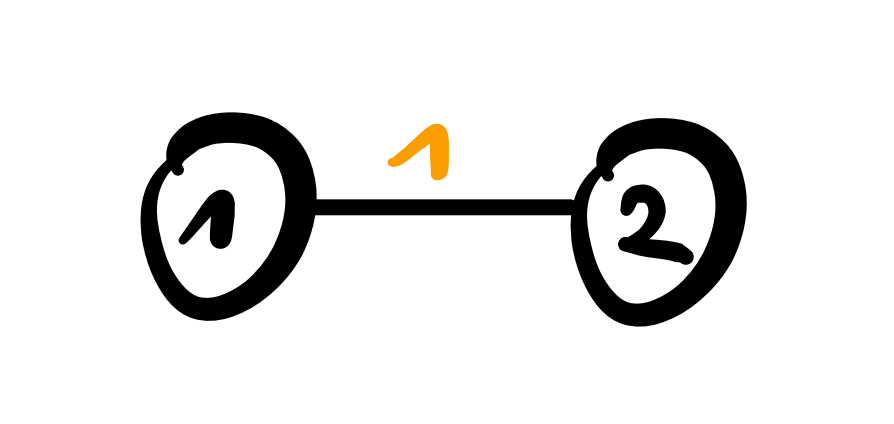
\includegraphics[width=3cm]{notes/figures/not_aperiodic.png}
\caption{Consider the initial distribution $\vp_0(1) = 1, \vp_0(2) = 0$. Clearly, the random walk will forever oscillate between the two states.}\label{fig:not_aperiodic}
\end{marginfigure}

We would also like to have that we converge to this stationary distribution regardless of the initial distribution $\vp_0$, but this is not true for general graphs, as is shown in \cref{fig:not_aperiodic}. A sufficient condition for convergence to the stationary distribution is, however, that all vertices have self-loops.\footnote{It is easy to check that this ensures that the Markov chain is aperiodic, which together with irreducibility implies convergence to the unique stationary distribution.}

Given the random walk $\mW$, the associated \emph{lazy random walk}\index{lazy random walk} is given by, \begin{align*}
    \Tilde{\mW} \defeq \frac{1}{2}\mI + \frac{1}{2}\mW,
\end{align*} that is, we add self-loops to each vertex with weight $\nicefrac{1}{2}$ and halve all other weights. Observe that this does not change the stationary distribution of the random walk. This ensures that the following holds.

\begin{thm}[Convergence of lazy random walk]\label{thm:convergence_of_lazy_random_walk}
For a connected graph, the lazy random walk converges to its unique stationary distribution irrespectively of the initial distribution $\vp_0$, \begin{align}
    \lim_{t\to\infty} \Tilde{\mW}^t\vp_0 = \Tilde{\vpi} = \vpi.
\end{align}
\end{thm}

To prove this theorem, let us first understand the transition matrix in terms of the graph Laplacian.

\begin{lem}
When $\nu_1, \dots, \nu_n$ are the eigenvalues and $\vpsi_1, \dots, \vpsi_n$ the corresponding eigenvectors of the normalized Laplacian matrix $\mN$, then $\Tilde{\mW}$ has eigenvalues $1 - \nicefrac{\nu_i}{2}$ and (not necessarily orthogonal) eigenvectors $\mD^{\nicefrac{1}{2}}\vpsi_i$.
\end{lem}\begin{proof} Let us first express the transition matrix of the original random walk in terms of the normalized graph Laplacian, \begin{align}
    \mW = \mA\inv{\mD} &= \mD^{\nicefrac{1}{2}}(\mD^{-\nicefrac{1}{2}}\mA\mD^{-\nicefrac{1}{2}})\mD^{-\nicefrac{1}{2}} \nonumber\\
    &= \mI + \mD^{\nicefrac{1}{2}}\underbrace{(\mD^{-\nicefrac{1}{2}}\mA\mD^{-\nicefrac{1}{2}} - \mI)}_{-\mN}\mD^{-\nicefrac{1}{2}} \nonumber\\
    &= \mI - \mD^{\nicefrac{1}{2}}\mN\mD^{-\nicefrac{1}{2}} \\
    &= \mD^{\nicefrac{1}{2}}(\mI - \mN)\mD^{-\nicefrac{1}{2}}. \nonumber
\end{align} By \cref{lem:a7}, $\mD^{\nicefrac{1}{2}}(\mI - \mN)\mD^{-\nicefrac{1}{2}}$ and $\mI - \mN$ have the same eigenvalues, namely $1 - \nu_i$. We also have, \begin{align}
    \Tilde{\mW} = \frac{1}{2}\mI + \frac{1}{2}(\mI - \mD^{\nicefrac{1}{2}}\mN\mD^{-\nicefrac{1}{2}}) = \mI - \frac{1}{2}\mD^{\nicefrac{1}{2}}\mN\mD^{-\nicefrac{1}{2}},
\end{align} implying that the eigenvalues of $\Tilde{\mW}$ are $1 - \nicefrac{\nu_i}{2}$. Finally, we have, \begin{align*}
    \Tilde{\mW}\mD^{\nicefrac{1}{2}}\vpsi_i &= (\mI - \frac{1}{2}\mD^{\nicefrac{1}{2}}\mN\mD^{-\nicefrac{1}{2}})\mD^{\nicefrac{1}{2}}\vpsi_i \\
    &= \mD^{\nicefrac{1}{2}}\vpsi_i - \frac{1}{2}\mD^{\nicefrac{1}{2}}\mN\vpsi_i \\
    &= \mD^{\nicefrac{1}{2}}\vpsi_i - \frac{\nu_i}{2}\mD^{\nicefrac{1}{2}}\vpsi_i \margintag{using that $\vpsi_i$ is an eigenvector of $\mN$ with corresponding eigenvalue $\nu_i$} \\
    &= \parentheses*{1 - \frac{\nu_i}{2}}\mD^{\nicefrac{1}{2}}\vpsi_i. \qedhere
\end{align*}
\end{proof}

\begin{proof}[Proof of \cref{thm:convergence_of_lazy_random_walk}]
TBD
\end{proof}

\begin{thm}[Convergence rate of lazy random walk]
For any unweighted connected graph $G$, we have that at time step $t$,\footnote{We will later see that $\nu_2$ is an indicator of the ``connectedness'' of $G$.} \begin{align}
    \norm{\vp_t - \vpi}_\infty \leq e^{-\nicefrac{\nu_2 t}{2}}\sqrt{n}.
\end{align}
\end{thm}
\begin{proof}
TBD
\end{proof}

\subsection{Hitting Time}

\begin{defn}[Hitting time] The \emph{hitting time}\index{hitting time}, \begin{align}
    H_{a,s} \defeq \min\{t \geq 1 \mid X_t = s, X_0 = a\},
\end{align} is the number of steps to reach $s$ starting from $a$. We have, \begin{align}
    \vh_s(a) \defeq \E{H_{a,s}} = 1 + \sum_{b \sim a} \frac{\vw(\{a,b\})}{\vd(a)} \vh_s(b). \label{eq:expected_hitting_time}
\end{align}
\end{defn}

\begin{lem}
If $\ex$ is a solution to $\mL\ex = \vd - \norm{\vd}_1 \vOne_s$,\footnote{We use $\vOne_s$ as a shorthand notation for $\vOne_{\{s\}}$.} then \begin{align}
    \vh_s = \ex - \ex(s)\vOne.
\end{align}
\end{lem}
\begin{proof}
For any $a \neq s$, we can equivalently write \cref{eq:expected_hitting_time} as, \begin{align*}
    \trans{\vOne_a}\vh_s = 1 + \trans{(\mW \vOne_a)}\vh_s \iff \trans{\vOne_a}(\mI - \trans{\mW})\vh_s = 1.
\end{align*} This yields a linear system of $n-1$ equations, \begin{align}
    \vOne - \alpha \vOne_s = (\mI - \underbrace{\trans{\mW}}_{\inv{\mD}\mA})\vh_s,
\end{align} where $\alpha$ is due to the remaining degree of freedom, as the entry corresponding to $s$ is not fixed. Multiplying from the left with $\mD$, we obtain, \begin{align*}
    \vd - \alpha \vd(s) \vOne_s = (\mD - \mA)\vh_s = \mL\vh_s.
\end{align*} Recall that $\ker{\mL} = \vspan\{\vOne\}$, and hence, for $\vh$ to exist, we must choose $\alpha$ such that $\vd - \alpha \vd(s) \vOne_s \perp \vOne$. We have, \begin{align*}
    \trans{\vOne}(\vd - \alpha \vd(s) \vOne_s) = \norm{\vd}_1 - \alpha \vd(s) \overset{!}{=} 0 \iff \alpha = \frac{\norm{\vd}_1}{\vd(s)}.
\end{align*} Finally, note that the solution $\ex$ to $\mL\ex = \vd - \norm{\vd}_1 \vOne_s$ is not unique. Given that $\vh_s$ is one solution, we have that any $\ex = \vh_s + c\vOne$ for $c \in \R$ is also a solution.\footnote{This follows directly from the fact that $\ker{\mL} = \vspan\{\vOne\}$.} Yet, we know that $\vh_s(s) = 0$, implying that $\vh_s = \ex - \ex(s)\vOne$.
\end{proof}

\subsection{Commute Time}

\begin{marginfigure}
TBD
% \centering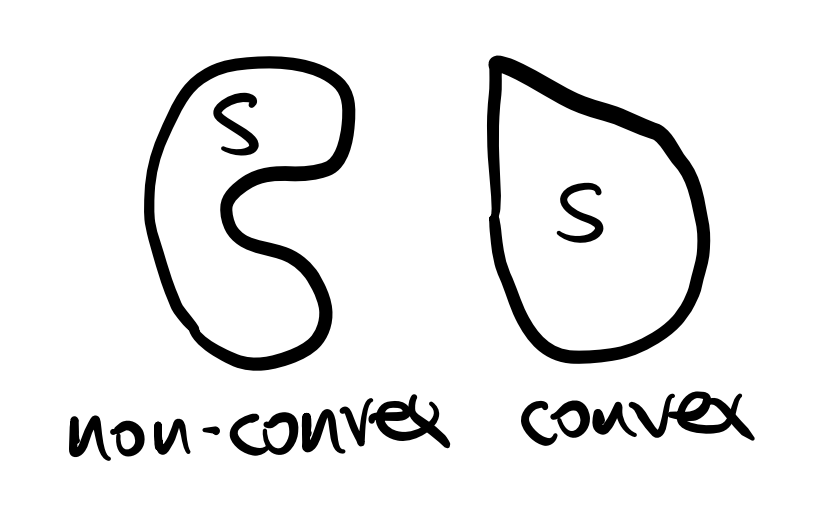
\includegraphics[width=4cm]{notes/figures/convex_set.png}
\caption{Example where hitting times are not symmetric.}
\end{marginfigure}
An issue with hitting times is that they do not need to be symmetric. This motivates the consideration of commute times, which correspond to the number of steps it takes to reach $b$ from $a$ and return to $a$.

\begin{defn}[Commute time] The \emph{commute time}\index{commute time} between $a$ and $b$ is defined as, \begin{align}
    C_{a,b} \defeq H_{a,b} + H_{b,a}.
\end{align}
\end{defn}
\begin{rmk}
By definition, commute times are symmetric.
\end{rmk}

\begin{lem}
If $\ex$ is a solution to $\mL\ex = \norm{\vd}_1 (\vOne_a - \vOne_b)$, then \begin{align}
    \E{C_{a,b}} = \trans{(\vOne_a - \vOne_b)}\ex = \ex(a) - \ex(b).
\end{align}
\end{lem} The $\ex$ can be interpreted as electrical voltages inducing flow that routes $\norm{\vd}_1$ units from $a$ to $b$.
\begin{proof}
We write $\vb_v \defeq \vd - \norm{\vd}_1 \vOne_v$ and let $\mL\ey = \vb_b$ and $\mL\ez = \vb_a$. Then, \begin{align*}
    \E{C_{a,b}} &= \vh_b(a) + \vh_a(b) \\
    &= \ey(a) - \ey(b) + \ez(b) - \ez(a) \\
    &= \trans{(\vOne_a - \vOne_b)}(\ey - \ez).
\end{align*} Observe that $\ex \defeq \ey - \ez$ solves $\mL\ex = \vb_b - \vb_a = \norm{\vd}_1 (\vOne_a - \vOne_b)$.
\end{proof}

We will see in \cref{cha:effective_resistance} that the expected commute time is intimately related to the electrical energy required to route flow from $a$ to $b$, also called the effective resistance between $a$ and $b$.

\section{Concentration}

\begin{thm}[Markov's inequality]\index{Markov's inequality}
For any random variable $X \geq 0$ and $t > 0$, \begin{align}
    \Pr{X \geq t} \leq \frac{\E{X}}{t}.
\end{align}
\end{thm}
\begin{proof} We have, \begin{align*}
    \E{X} = \int_0^\infty x f(x) \,dx \geq \int_t^\infty x f(x) \, dx \geq t \int_t^\infty f(x) \,dx = t \Pr{X \geq t},
\end{align*} where $f$ is the probability density function of $X$.
\end{proof}

\begin{thm}[Jensen's inequality]\index{Jensen's inequality}
For a random variable $X$, if $f$ is convex, then $\E{f(X)} \geq f(\E{X})$.\footnote{Proof of the finite form in \cref{thm:a8}.}
\end{thm}
\begin{marginfigure}
TBD
% \centering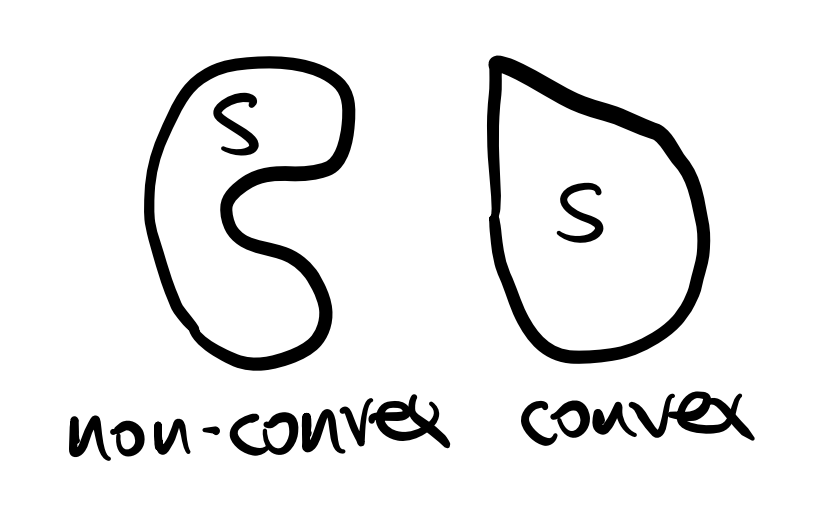
\includegraphics[width=4cm]{notes/figures/convex_set.png}
\caption{Jensen's inequality.}
\end{marginfigure}

\begin{thm}[Bernstein concentration bound]\index{Bernstein concentration bound} Given independent real-valued random variables $X_1, \dots, X_k \in \R$ such that $\E{X_i} = 0$ and $|X_i| \leq R$. Let $X \defeq \sum_i X_i$ and $\sigma^2 \defeq \Var{X} = \sum_i \E{X_i^2}$. Then, for $t > 0$, \begin{align}
    \Pr{|X| \geq t} \leq 2 \exp\parentheses*{\frac{-t^2}{2Rt + 4\sigma^2}}.
\end{align}
\end{thm}
\begin{proof}
TBD
\end{proof}

\begin{thm}[Bernstein matrix concentration bound]\index{Bernstein matrix concentration bound} Suppose $\rX_1, \dots, \rX_k \in \R^{n \times n}$ are independent symmetric matrix-valued random variables satisfying $\E{\rX_i} = \mZero$ and $\norm{\rX_i}_2 \leq R$. Let $\rX \defeq \sum_i \rX_i$ and $\sigma^2 \defeq \Var{\rX} = \sum_i \E{\rX_i^2}$. Then, for $t > 0$, \begin{align}
    \Pr{\norm{\rX}_2 \geq t} \leq 2 n \exp\parentheses*{\frac{-t^2}{2Rt + 4\sigma^2}}.
\end{align}
\end{thm}
\begin{proof}
TBD
\end{proof}

\section{Martingales}

\begin{defn}[Martingale] A \emph{martingale}\index{martingale} is a sequence of random variables $Z_0, \dots, Z_k$ such that \begin{align}
    \E{Z_i \mid Z_0, \dots, Z_{i-1}} = Z_{i-1}.
\end{align} That is, conditional on the outcome of all the previous random variables, the expectation of $Z_i$ equals $Z_{i-1}$.% In particular, $\E{Z_k} = \E{Z_0}$.
\end{defn} Typically, we use martingales to show a statement such as ``$Z_k$ is concentrated around $\E{Z_k}$''.

We can alternatively think of a martingale as the sequence of changes in $Z_i$. Let $X_i \defeq Z_i - Z_{i-1}$. The sequence of $X_i$ is called \emph{martingale difference sequence}\index{martingale difference sequence}. The martingale condition is equivalent to, \begin{align}
    \E{X_i \mid Z_0, \dots, Z_{i-1}} = \E{X_i \mid Z_0, X_1, \dots, X_{i-1}} = 0.
\end{align} We can write, \begin{align}
    Z_k = Z_0 + \sum_{i=1}^k Z_i - Z_{i-1} = Z_0 + \sum_{i=1}^k X_i.
\end{align}